% Options for packages loaded elsewhere
% Options for packages loaded elsewhere
\PassOptionsToPackage{unicode}{hyperref}
\PassOptionsToPackage{hyphens}{url}
\PassOptionsToPackage{dvipsnames,svgnames,x11names}{xcolor}
%
\documentclass[
  italian,
  letterpaper,
  DIV=11,
  numbers=noendperiod]{scrreprt}
\usepackage{xcolor}
\usepackage{amsmath,amssymb}
\setcounter{secnumdepth}{5}
\usepackage{iftex}
\ifPDFTeX
  \usepackage[T1]{fontenc}
  \usepackage[utf8]{inputenc}
  \usepackage{textcomp} % provide euro and other symbols
\else % if luatex or xetex
  \usepackage{unicode-math} % this also loads fontspec
  \defaultfontfeatures{Scale=MatchLowercase}
  \defaultfontfeatures[\rmfamily]{Ligatures=TeX,Scale=1}
\fi
\usepackage{lmodern}
\ifPDFTeX\else
  % xetex/luatex font selection
\fi
% Use upquote if available, for straight quotes in verbatim environments
\IfFileExists{upquote.sty}{\usepackage{upquote}}{}
\IfFileExists{microtype.sty}{% use microtype if available
  \usepackage[]{microtype}
  \UseMicrotypeSet[protrusion]{basicmath} % disable protrusion for tt fonts
}{}
\makeatletter
\@ifundefined{KOMAClassName}{% if non-KOMA class
  \IfFileExists{parskip.sty}{%
    \usepackage{parskip}
  }{% else
    \setlength{\parindent}{0pt}
    \setlength{\parskip}{6pt plus 2pt minus 1pt}}
}{% if KOMA class
  \KOMAoptions{parskip=half}}
\makeatother
% Make \paragraph and \subparagraph free-standing
\makeatletter
\ifx\paragraph\undefined\else
  \let\oldparagraph\paragraph
  \renewcommand{\paragraph}{
    \@ifstar
      \xxxParagraphStar
      \xxxParagraphNoStar
  }
  \newcommand{\xxxParagraphStar}[1]{\oldparagraph*{#1}\mbox{}}
  \newcommand{\xxxParagraphNoStar}[1]{\oldparagraph{#1}\mbox{}}
\fi
\ifx\subparagraph\undefined\else
  \let\oldsubparagraph\subparagraph
  \renewcommand{\subparagraph}{
    \@ifstar
      \xxxSubParagraphStar
      \xxxSubParagraphNoStar
  }
  \newcommand{\xxxSubParagraphStar}[1]{\oldsubparagraph*{#1}\mbox{}}
  \newcommand{\xxxSubParagraphNoStar}[1]{\oldsubparagraph{#1}\mbox{}}
\fi
\makeatother


\usepackage{longtable,booktabs,array}
\newcounter{none} % for unnumbered tables
\usepackage{calc} % for calculating minipage widths
% Correct order of tables after \paragraph or \subparagraph
\usepackage{etoolbox}
\makeatletter
\patchcmd\longtable{\par}{\if@noskipsec\mbox{}\fi\par}{}{}
\makeatother
% Allow footnotes in longtable head/foot
\IfFileExists{footnotehyper.sty}{\usepackage{footnotehyper}}{\usepackage{footnote}}
\makesavenoteenv{longtable}
\usepackage{graphicx}
\makeatletter
\newsavebox\pandoc@box
\newcommand*\pandocbounded[1]{% scales image to fit in text height/width
  \sbox\pandoc@box{#1}%
  \Gscale@div\@tempa{\textheight}{\dimexpr\ht\pandoc@box+\dp\pandoc@box\relax}%
  \Gscale@div\@tempb{\linewidth}{\wd\pandoc@box}%
  \ifdim\@tempb\p@<\@tempa\p@\let\@tempa\@tempb\fi% select the smaller of both
  \ifdim\@tempa\p@<\p@\scalebox{\@tempa}{\usebox\pandoc@box}%
  \else\usebox{\pandoc@box}%
  \fi%
}
% Set default figure placement to htbp
\def\fps@figure{htbp}
\makeatother



\ifLuaTeX
\usepackage[bidi=basic,shorthands=off]{babel}
\else
\usepackage[bidi=default,shorthands=off]{babel}
\fi
\ifLuaTeX
  \usepackage{selnolig} % disable illegal ligatures
\fi


\setlength{\emergencystretch}{3em} % prevent overfull lines

\providecommand{\tightlist}{%
  \setlength{\itemsep}{0pt}\setlength{\parskip}{0pt}}



 


\KOMAoption{captions}{tableheading}
\makeatletter
\@ifpackageloaded{tcolorbox}{}{\usepackage[skins,breakable]{tcolorbox}}
\@ifpackageloaded{fontawesome5}{}{\usepackage{fontawesome5}}
\definecolor{quarto-callout-color}{HTML}{909090}
\definecolor{quarto-callout-note-color}{HTML}{0758E5}
\definecolor{quarto-callout-important-color}{HTML}{CC1914}
\definecolor{quarto-callout-warning-color}{HTML}{EB9113}
\definecolor{quarto-callout-tip-color}{HTML}{00A047}
\definecolor{quarto-callout-caution-color}{HTML}{FC5300}
\definecolor{quarto-callout-color-frame}{HTML}{acacac}
\definecolor{quarto-callout-note-color-frame}{HTML}{4582ec}
\definecolor{quarto-callout-important-color-frame}{HTML}{d9534f}
\definecolor{quarto-callout-warning-color-frame}{HTML}{f0ad4e}
\definecolor{quarto-callout-tip-color-frame}{HTML}{02b875}
\definecolor{quarto-callout-caution-color-frame}{HTML}{fd7e14}
\makeatother
\makeatletter
\@ifpackageloaded{bookmark}{}{\usepackage{bookmark}}
\makeatother
\makeatletter
\@ifpackageloaded{caption}{}{\usepackage{caption}}
\AtBeginDocument{%
\ifdefined\contentsname
  \renewcommand*\contentsname{Indice}
\else
  \newcommand\contentsname{Indice}
\fi
\ifdefined\listfigurename
  \renewcommand*\listfigurename{Elenco delle Figure}
\else
  \newcommand\listfigurename{Elenco delle Figure}
\fi
\ifdefined\listtablename
  \renewcommand*\listtablename{Elenco delle Tabelle}
\else
  \newcommand\listtablename{Elenco delle Tabelle}
\fi
\ifdefined\figurename
  \renewcommand*\figurename{Figura}
\else
  \newcommand\figurename{Figura}
\fi
\ifdefined\tablename
  \renewcommand*\tablename{Tabella}
\else
  \newcommand\tablename{Tabella}
\fi
}
\@ifpackageloaded{float}{}{\usepackage{float}}
\floatstyle{ruled}
\@ifundefined{c@chapter}{\newfloat{codelisting}{h}{lop}}{\newfloat{codelisting}{h}{lop}[chapter]}
\floatname{codelisting}{Lista}
\newcommand*\listoflistings{\listof{codelisting}{Elenco degli Elenchi}}
\makeatother
\makeatletter
\makeatother
\makeatletter
\@ifpackageloaded{caption}{}{\usepackage{caption}}
\@ifpackageloaded{subcaption}{}{\usepackage{subcaption}}
\makeatother
\usepackage{bookmark}
\IfFileExists{xurl.sty}{\usepackage{xurl}}{} % add URL line breaks if available
\urlstyle{same}
% fallback for those not using the hyperref driver hyperxmp:
\makeatletter
\@ifundefined{xmpquote}{\newcommand{\xmpquote}[1]{#1}}{}
\makeatother
\hypersetup{
  pdftitle={Lab1: misure e statistica},
  pdfauthor={Progetto Lab1},
  pdflang={it},
  colorlinks=true,
  linkcolor={blue},
  filecolor={Maroon},
  citecolor={Blue},
  urlcolor={Blue},
  pdfcreator={LaTeX via pandoc}}


\title{Lab1: misure e statistica}
\usepackage{etoolbox}
\makeatletter
\providecommand{\subtitle}[1]{% add subtitle to \maketitle
  \apptocmd{\@title}{\par {\large #1 \par}}{}{}
}
\makeatother
\subtitle{Dispensa essenziale · Capitolo pilota}
\author{Progetto Lab1}
\date{}
\begin{document}
\maketitle

\renewcommand*\contentsname{Indice}
{
\setcounter{tocdepth}{2}
\tableofcontents
}

\bookmarksetup{startatroot}

\chapter*{Come leggere questa
dispensa}\label{come-leggere-questa-dispensa}
\addcontentsline{toc}{chapter}{Come leggere questa dispensa}

\markboth{Come leggere questa dispensa}{Come leggere questa dispensa}

Questa dispensa accompagna il laboratorio di Fisica 1: mette in evidenza
\textbf{che cosa descrive un modello, quando si può usare e come
interpretare un risultato}.

Il primo capitolo è dedicato alla distribuzione binomiale. Si parte da
una domanda concreta: quante volte può verificarsi un certo esito,
ripetendo una prova?

\begin{tcolorbox}[enhanced jigsaw, arc=.35mm, bottomrule=.15mm, bottomtitle=1mm, breakable, colback=white, colbacktitle=quarto-callout-note-color!10!white, colframe=quarto-callout-note-color-frame, coltitle=black, left=2mm, leftrule=.75mm, opacityback=0, opacitybacktitle=0.6, rightrule=.15mm, title={Un percorso in tre passi}, titlerule=0mm, toprule=.15mm, toptitle=1mm]

\begin{enumerate}
\def\labelenumi{\arabic{enumi}.}
\tightlist
\item
  \textbf{Capisci il modello.} Identifica la grandezza che varia e le
  ipotesi.
\item
  \textbf{Usalo.} Segui un esempio e interpreta il numero ottenuto.
\item
  \textbf{Verifica.} Fai una previsione, esplora la simulazione e
  confronta.
\end{enumerate}

\end{tcolorbox}

I riquadri \textbf{Da ricordare} raccolgono i risultati essenziali;
\textbf{Attenzione} segnala gli errori frequenti. Gli approfondimenti
sono separati dal percorso principale. Nella versione HTML puoi
sperimentare direttamente; il PDF contiene gli stessi concetti, gli
esempi, una figura statica e le domande dell'attività.

\section*{Fonte e attribuzione}\label{fonte-e-attribuzione}
\addcontentsline{toc}{section}{Fonte e attribuzione}

\markright{Fonte e attribuzione}

Il capitolo è una rielaborazione sintetica dei contenuti sulla binomiale
e sulle misure di efficienza di \emph{Introduzione all'analisi dei dati.
Per il laboratorio di Fisica}, di \textbf{Luca Baldini, Niccolò Di
Lalla, Massimiliano Razzano e Carmelo Sgrò}, disponibile nel
\href{https://github.com/unipi-physics-labs/lab1-notes}{progetto
lab1-notes}.

Testo riorganizzato e abbreviato; figura e attività interattiva aggiunte
per questo percorso. L'opera originale e questo adattamento sono
distribuiti con licenza
\href{https://creativecommons.org/licenses/by-sa/4.0/}{Creative Commons
Attribuzione - Condividi allo stesso modo 4.0}.

\bookmarksetup{startatroot}

\chapter{La distribuzione binomiale}\label{sec-binomiale}

\begin{tcolorbox}[enhanced jigsaw, arc=.35mm, bottomrule=.15mm, bottomtitle=1mm, breakable, colback=white, colbacktitle=quarto-callout-note-color!10!white, colframe=quarto-callout-note-color-frame, coltitle=black, left=2mm, leftrule=.75mm, opacityback=0, opacitybacktitle=0.6, rightrule=.15mm, title={Alla fine del capitolo sai\ldots{}}, titlerule=0mm, toprule=.15mm, toptitle=1mm]

\begin{itemize}
\tightlist
\item
  riconoscere quando un conteggio segue una distribuzione binomiale;
\item
  distinguere numero di prove, numero di successi e numero di serie;
\item
  calcolare una probabilità e interpretare media e deviazione standard;
\item
  spiegare che cosa cambia quando aumentano i dati raccolti.
\end{itemize}

\end{tcolorbox}

\section{Che cosa stiamo contando?}\label{che-cosa-stiamo-contando}

Lanciamo un dado cento volte e contiamo quante volte esce \textbf{la
faccia 1}. In questo esempio definiamo \emph{successo} l'uscita di 1 e
\emph{insuccesso} l'uscita di una delle altre cinque facce. Se il dado è
equo, la probabilità di successo è \(p=1/6\).

Una \textbf{prova} è un singolo lancio. Una \textbf{serie} comprende
\(n\) prove. Il risultato della serie è il conteggio \(k\): il numero di
successi osservati.

{\def\LTcaptype{none} % do not increment counter
\begin{longtable}[]{@{}cll@{}}
\toprule\noalign{}
Simbolo & Significato & Esempio del dado \\
\midrule\noalign{}
\endhead
\bottomrule\noalign{}
\endlastfoot
\(n\) & Numero di prove in una serie & 100 lanci \\
\(p\) & Probabilità di successo in ogni prova & \(1/6\) \\
\(k\) & Numero di successi nella serie & Quante volte esce 1 \\
\(M\) & Numero di serie simulate & Quante serie di 100 lanci
ripetiamo \\
\end{longtable}
}

\(n\) e \(p\) definiscono la distribuzione. \(k\) è la variabile
casuale, che può valere \(0,1,\ldots,n\). \(M\) indica quanti conteggi
raccogliamo nella simulazione; complessivamente eseguiamo \(nM\) prove.

\begin{tcolorbox}[enhanced jigsaw, arc=.35mm, bottomrule=.15mm, bottomtitle=1mm, breakable, colback=white, colbacktitle=quarto-callout-important-color!10!white, colframe=quarto-callout-important-color-frame, coltitle=black, left=2mm, leftrule=.75mm, opacityback=0, opacitybacktitle=0.6, rightrule=.15mm, title={Quando si applica}, titlerule=0mm, toprule=.15mm, toptitle=1mm]

Il numero di successi segue una binomiale se \textbf{il numero di prove
è fissato}, le prove sono \textbf{indipendenti}, ciascuna è classificata
in \textbf{successo o insuccesso} e la probabilità \(p\) è \textbf{la
stessa in ogni prova}.

\end{tcolorbox}

La definizione di successo dipende dalla domanda: per una moneta può
essere «esce testa»; per un rivelatore, «la particella produce un
segnale». Avere due categorie di esito, da solo, non basta a garantire
il modello binomiale.

\section{La probabilità di un
conteggio}\label{la-probabilituxe0-di-un-conteggio}

La probabilità di ottenere \textbf{esattamente \(k\) successi} è

\begin{equation}\protect\phantomsection\label{eq-binomiale}{
B(k;n,p)=\binom{n}{k}p^k(1-p)^{n-k},
\qquad \binom{n}{k}=\frac{n!}{k!(n-k)!}.
}\end{equation}

Una particolare sequenza con \(k\) successi ha probabilità
\(p^k(1-p)^{n-k}\). Il coefficiente binomiale conta quante sequenze
diverse hanno quel numero di successi. Sommando le probabilità di queste
sequenze si ottiene Equazione~\ref{eq-binomiale}.

\subsection{Esempio: due teste in quattro
lanci}\label{esempio-due-teste-in-quattro-lanci}

Per una moneta equa, \(n=4\) e \(p=1/2\). Tra le 16 sequenze possibili,
tutte equiprobabili, sei contengono due teste:

\[
B(2;4,1/2)=\binom{4}{2}\left(\frac12\right)^4
=\frac{6}{16}=0{,}375.
\]

\textbf{Interpretazione:} ripetendo molte serie di quattro lanci, la
frazione di serie con esattamente due teste tende al 37,5\%.

\subsection{Eventi che comprendono più
conteggi}\label{eventi-che-comprendono-piuxf9-conteggi}

Per «al massimo tre successi» si sommano quattro probabilità:

\[
P(k\leq 3)=\sum_{j=0}^{3}B(j;n,p).
\]

Per «almeno un successo» è più rapido usare l'evento complementare:

\[
P(k\geq1)=1-P(k=0)=1-(1-p)^n.
\]

\begin{tcolorbox}[enhanced jigsaw, arc=.35mm, bottomrule=.15mm, bottomtitle=1mm, breakable, colback=white, colbacktitle=quarto-callout-warning-color!10!white, colframe=quarto-callout-warning-color-frame, coltitle=black, left=2mm, leftrule=.75mm, opacityback=0, opacitybacktitle=0.6, rightrule=.15mm, title={Attenzione: esattamente e almeno sono eventi diversi}, titlerule=0mm, toprule=.15mm, toptitle=1mm]

\(B(3;n,p)\) riguarda solo \(k=3\). La probabilità \(P(k\geq3)\)
comprende tutti i conteggi da 3 a \(n\). Prima di calcolare, traduci la
domanda in un evento preciso.

\end{tcolorbox}

\section{Media, dispersione e precisione della
media}\label{media-dispersione-e-precisione-della-media}

\begin{tcolorbox}[enhanced jigsaw, arc=.35mm, bottomrule=.15mm, bottomtitle=1mm, breakable, colback=white, colbacktitle=quarto-callout-note-color!10!white, colframe=quarto-callout-note-color-frame, coltitle=black, left=2mm, leftrule=.75mm, opacityback=0, opacitybacktitle=0.6, rightrule=.15mm, title={Da ricordare}, titlerule=0mm, toprule=.15mm, toptitle=1mm]

Per una binomiale:

\[
\mu=np,\qquad \sigma^2=np(1-p),\qquad \sigma=\sqrt{np(1-p)}.
\]

\(\mu\) è il numero medio di successi per serie. \(\sigma\) descrive la
dispersione dei conteggi delle singole serie attorno alla media.

\end{tcolorbox}

Per quattro lanci di moneta equa, \(\mu=2\) e \(\sigma=1\). Per cento
lanci di dado equo, contando la faccia 1, \(\mu\simeq16{,}67\) e
\(\sigma\simeq3{,}73\). La media non deve essere intera, anche se ogni
conteggio lo è.

\begin{figure}

\centering{

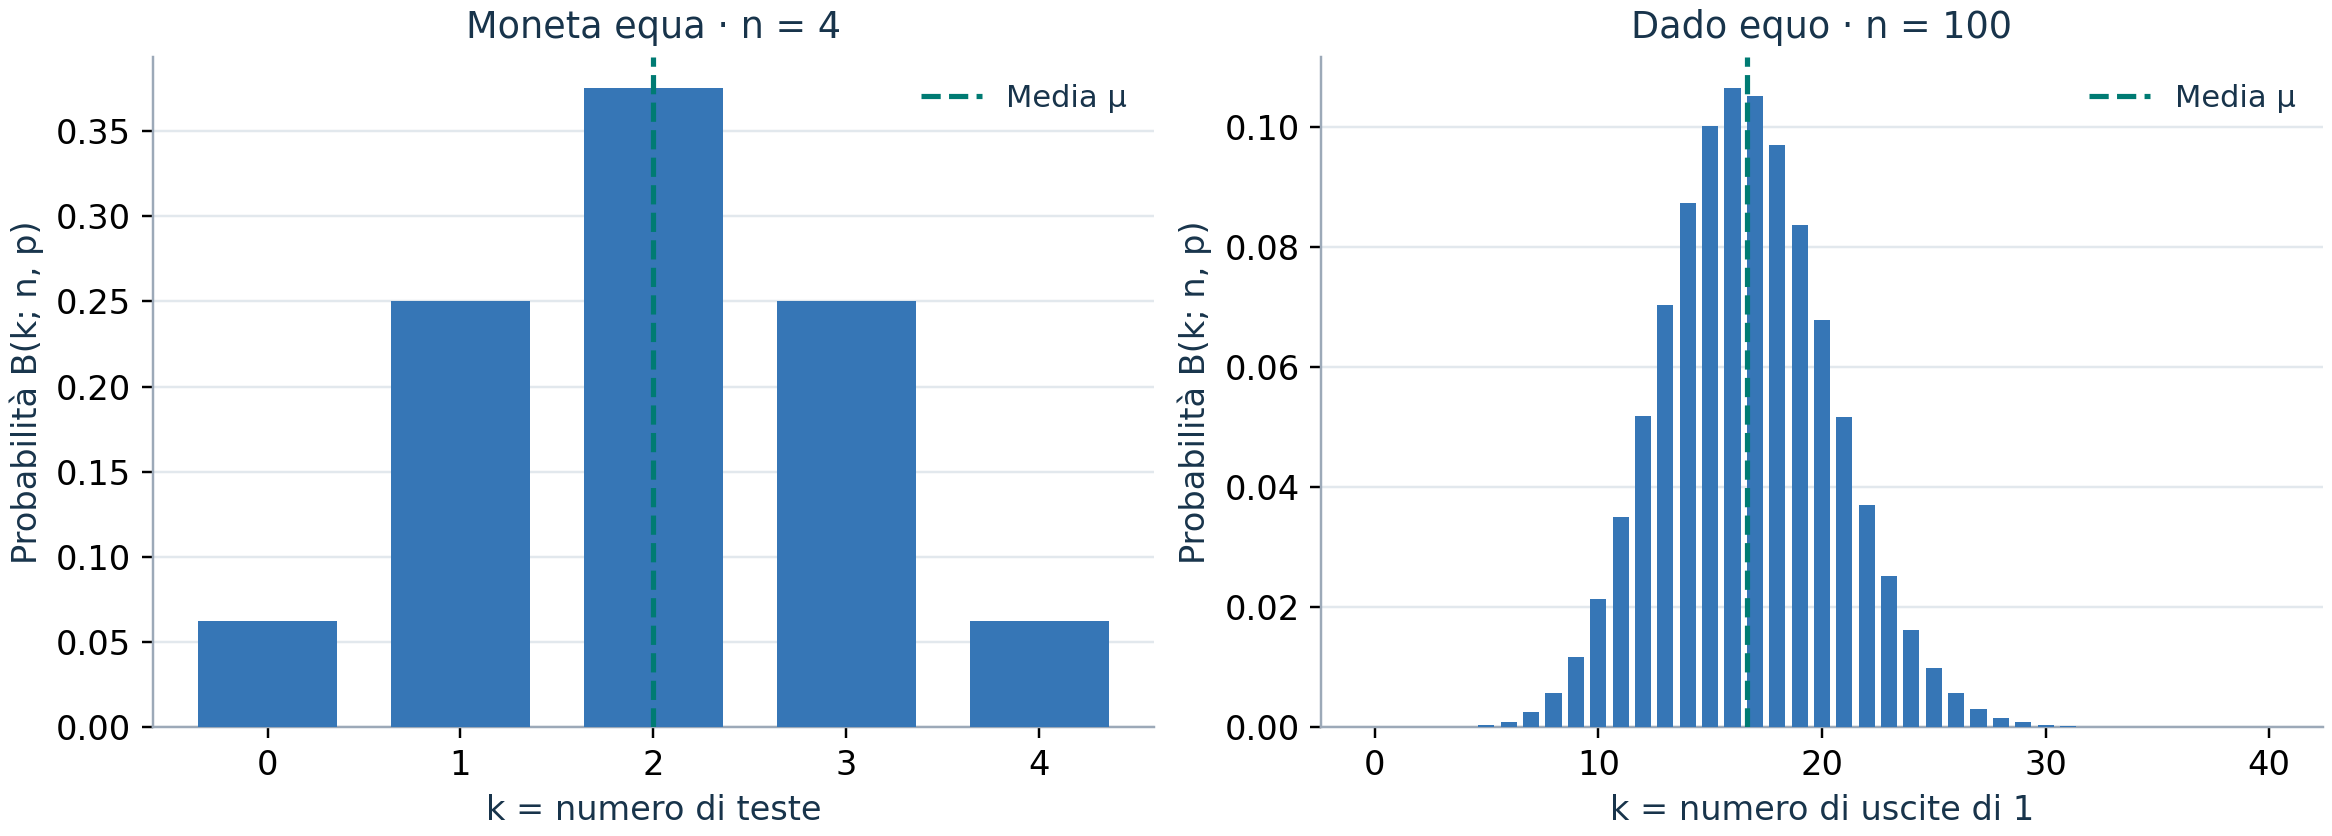
\includegraphics[width=1\linewidth,height=\textheight,keepaspectratio,alt={Probabilità discrete per la moneta, simmetriche attorno a 2, e per il dado, concentrate attorno a 16,7.}]{capitoli/../immagini/binomiale_confronto.png}

}

\caption{\label{fig-confronto}Due esempi di binomiale. A sinistra:
numero di teste in quattro lanci di moneta equa. A destra: numero di
uscite della faccia 1 in cento lanci di dado equo; sono mostrati i
conteggi da 0 a 40, oltre i quali la probabilità è trascurabile alla
scala del grafico. La linea tratteggiata indica la media.}

\end{figure}%

Se ripetiamo la serie \(M\) volte, otteniamo \(k_1,\ldots,k_M\) e la
media campionaria \(\bar{k}=M^{-1}\sum_{i=1}^M k_i\). Per serie
indipendenti con gli stessi \(n,p\):

\[
\sigma_{\bar{k}}=\frac{\sigma}{\sqrt M}.
\]

Se \(\sigma\) non è nota, la stimiamo con \(s\), dove
\(s^2=\sum_{i=1}^M(k_i-\bar{k})^2/(M-1)\) per \(M\geq2\): la stima
dell'incertezza sulla media è \(s/\sqrt M\).

\textbf{Aumentare \(M\) rende più precisa la media; non restringe la
distribuzione dei singoli conteggi.} A \(n,p\) fissati, \(\sigma\)
rimane la stessa. La stima \(s\) fluttua al cambiare del campione e non
deve aumentare o diminuire in modo monotono.

\section{Un risultato raro: tre ``1'' in cento
lanci}\label{un-risultato-raro-tre-1-in-cento-lanci}

Per un dado equo, la probabilità di osservare al massimo tre uscite
della faccia 1 in cento lanci vale

\[
P(k\leq3)=\sum_{j=0}^{3}B(j;100,1/6)
\simeq1{,}83\times10^{-5}.
\]

È circa lo \textbf{0,00183\%}. Un risultato così basso è molto raro
sotto l'ipotesi di dado equo e lanci indipendenti. Questo calcolo
\textbf{non} è la probabilità che il dado sia equo: descrive i risultati
attesi assumendo quel modello.

Una simulazione di poche migliaia di serie può non produrre alcun caso
di questo tipo. Una frequenza osservata nulla non implica una
probabilità teorica nulla.

\section{Prova tu: dalla previsione ai dati}\label{sec-attivita}

Prima di simulare, scrivi una previsione; poi confrontala con il
risultato.

\begin{enumerate}
\def\labelenumi{\arabic{enumi}.}
\tightlist
\item
  \textbf{Moneta.} Scegli il pulsante «Moneta»: imposta \(n=4\),
  \(p=1/2\) ed «esattamente 2». Simula 100 serie, poi aggiungine 1.000.
  La frequenza si avvicina a 0,375? Può allontanarsene temporaneamente?
\item
  \textbf{Dispersione.} Lascia fissi \(n,p\) e aumenta \(M\). Confronta
  \(s\) e \(s/\sqrt M\): quale grandezza descrive la variabilità di una
  singola serie?
\item
  \textbf{Dado.} Scegli il pulsante «Dado»: imposta \(n=100\), \(p=1/6\)
  e «al massimo 3». Confronta probabilità teorica e frequenza simulata.
  Come interpreti zero casi osservati?
\end{enumerate}

\begin{tcolorbox}[enhanced jigsaw, arc=.35mm, bottomrule=.15mm, bottomtitle=1mm, breakable, colback=white, colbacktitle=quarto-callout-tip-color!10!white, colframe=quarto-callout-tip-color-frame, coltitle=black, left=2mm, leftrule=.75mm, opacityback=0, opacitybacktitle=0.6, rightrule=.15mm, title={Attività interattiva}, titlerule=0mm, toprule=.15mm, toptitle=1mm]

Nella versione HTML di questo capitolo trovi la simulazione. Se hai la
cartella del progetto, puoi aprire anche il file
\texttt{interattivi/binomiale\_lab1.html} nel browser. La
Figura~\ref{fig-confronto} mostra le distribuzioni teoriche su cui
basare le previsioni.

\end{tcolorbox}

\begin{tcolorbox}[enhanced jigsaw, arc=.35mm, bottomrule=.15mm, bottomtitle=1mm, breakable, colback=white, colbacktitle=quarto-callout-tip-color!10!white, colframe=quarto-callout-tip-color-frame, coltitle=black, left=2mm, leftrule=.75mm, opacityback=0, opacitybacktitle=0.6, rightrule=.15mm, title={Confronta le tue risposte}, titlerule=0mm, toprule=.15mm, toptitle=1mm]

La frequenza tende alla probabilità teorica, ma il suo avvicinamento non
è monotono. \(s\) stima la dispersione delle singole serie;
\(s/\sqrt M\) stima la precisione della loro media. Un evento molto raro
può non comparire in un campione finito: il calcolo teorico resta
diverso da zero.

\end{tcolorbox}

\section{Un'applicazione: misurare
un'efficienza}\label{unapplicazione-misurare-unefficienza}

Un rivelatore produce un segnale per 962 delle 1.000 particelle
incidenti. Definendo il successo come «segnale prodotto», abbiamo
\(n=1000\) prove e \(k=962\) successi. Stimiamo l'efficienza con la
frazione osservata:

\[
\hat\varepsilon=\frac{k}{n}=0{,}962,
\qquad
s_{\hat\varepsilon}=\sqrt{\frac{\hat\varepsilon(1-\hat\varepsilon)}{n}}
\simeq0{,}006.
\]

Questa stima dell'errore è utile quando successi e insuccessi sono
entrambi abbastanza numerosi. Per \(k=0\) o \(k=n\) restituisce zero:
\textbf{non significa che l'efficienza sia nota esattamente}. Il
problema richiede una trattazione diversa.

\begin{tcolorbox}[enhanced jigsaw, arc=.35mm, bottomrule=.15mm, bottomtitle=1mm, breakable, colback=white, colbacktitle=quarto-callout-note-color!10!white, colframe=quarto-callout-note-color-frame, coltitle=black, left=2mm, leftrule=.75mm, opacityback=0, opacitybacktitle=0.6, rightrule=.15mm, title={Approfondimento: perché media e varianza hanno questa forma}, titlerule=0mm, toprule=.15mm, toptitle=1mm]

Scriviamo il conteggio come somma \(k=Y_1+\cdots+Y_n\), con \(Y_i=1\)
per un successo e \(Y_i=0\) per un insuccesso. Ogni \(Y_i\) ha media
\(p\) e varianza \(p(1-p)\). Le medie si sommano; per prove indipendenti
si sommano anche le varianze. Quindi \(E[k]=np\) e
\(\mathrm{Var}(k)=np(1-p)\).

\end{tcolorbox}

\begin{tcolorbox}[enhanced jigsaw, arc=.35mm, bottomrule=.15mm, bottomtitle=1mm, breakable, colback=white, colbacktitle=quarto-callout-important-color!10!white, colframe=quarto-callout-important-color-frame, coltitle=black, left=2mm, leftrule=.75mm, opacityback=0, opacitybacktitle=0.6, rightrule=.15mm, title={Prima di passare oltre}, titlerule=0mm, toprule=.15mm, toptitle=1mm]

Sai definire il successo prima di guardare il grafico? Sai distinguere
\(n\), \(k\) e \(M\)? Sai spiegare perché una media più precisa non
implica conteggi meno dispersi? Se sì, hai acquisito le idee centrali
del capitolo.

\end{tcolorbox}




\end{document}
